\input{/home/pantoufle/cours/Perso/Commun/macros_TD.tex}

\title{Inpainting - CGDI}

\author{Simon \textsc{Fernandez}}
\date{\today}

\begin{document}
\maketitle

\section{L'algorithme}
Suite à quelques recherches, j'ai décidé d'implémenter la méthode 
décrite dans l'article Object removal by exemblar-based inpainting
\cite{article}.

Le principe de l'algorithme est de remplire la zone à colorer avec des 
patchs venant d'autres parts de l'image, venant de la zone à garder.
L'algorithme remplit la zone en commençant par les frontières, et après
application des patchs, cette frontière recule de plus en plus, jusqu'à 
ce que toute la zone à completer soit colorée. 

Lors de la coloration d'une zone frontalière, l'algorithme choisit le 
patch dans l'image minimisant la distance avec la zone connue de la zone
à colorer. Ainsi, la frontière est colorée avec des pixels dont le voisinage
ressemble au voisinage de la frontière. On a donc une coloration avec 
des patchs d'image connue, et donc considérés comme connus et bons.

L'algorithme ne choisit pas la zone frontalière à colorer au hasard. En 
effet, un indice de confiance est donné à chaque pixel. Plus un pixel 
est proche d'une zone connue, d'une partie de l'image qu'on connait déjà,
plus sa confiance est élevée, plus l'algorithme aura tendance à le 
sélectionner pour l'étape de remplissage. 

Ce qui distingue cet article\cite{article}, c'est qu'il ajoute le gradient
de la frontière pour pousser l'algorithme à remplir en priorité les 
points de la frontière dans la continuité d'un fort gradient. En effet,
ces forts gradients sont causés par des formes géométriques dans la figure,
par exemple la ligne d'horizon, un trotoire, etc...
Ces figures géométriques ayant de fortes chances d'être prolongées, on peut
les remplire en priorité. Ainsi, en prenant une combinaison de la confiance
et de ces lignes géométriques, l'algorithme aura tendance à fournir une 
image plus cohérente.

\section{Points forts}
\subsection{Le flou}
Cet algorithme fait des copiers collers de zones préexistantes, il évite
ainsi l'impression de flou que donnent d'autres algorithmes qui calculent
la valeur du pixel à completer, les zones complétées sont nettes et 
correspondent au style de l'image de départ.

\begin{figure}[ht]
\centering
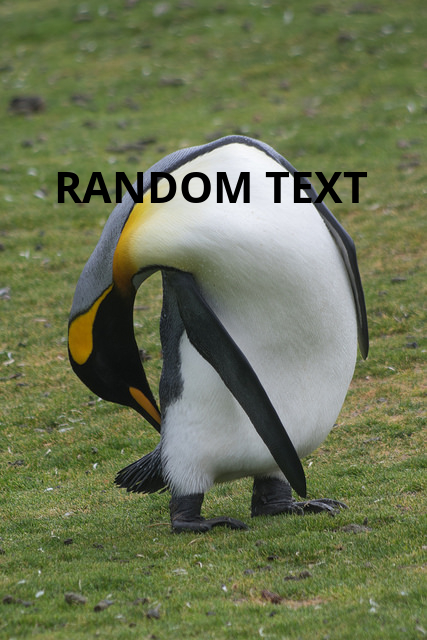
\includegraphics[height=7.5cm]{img/examples/penguin.jpg}
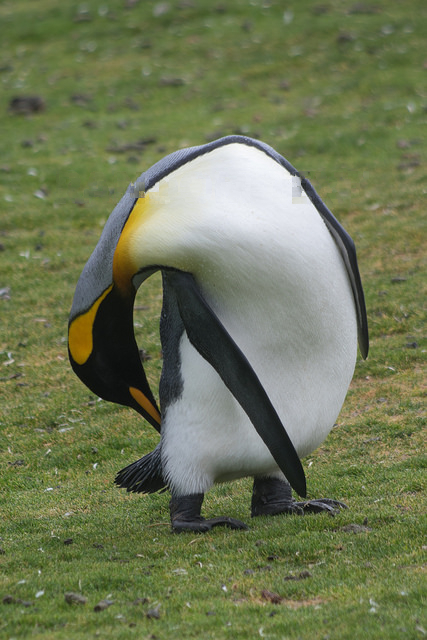
\includegraphics[height=7.5cm]{img/examples/penguin_res.jpg}
\caption{Effacement de texte}
\end{figure}

\subsection{Le style}
Comme l'algorithme copie des zones prééxistantes, le style, luminosité, tons
de l'image de départ sont conservés. En effet, si on donne en entrée une
image dessinée, le résultat gardera cette impression de dessin puisque tous
les pixels ajoutés viendront d'un dessin. 
De la même façon, le ton de l'image est conservé. Dans le cas d'une forêt 
brumeuse avec des tons gris-bleus, ce sont ces mêmes pixels qui seront 
ajoutés à l'image.

\begin{figure}[ht]
\centering
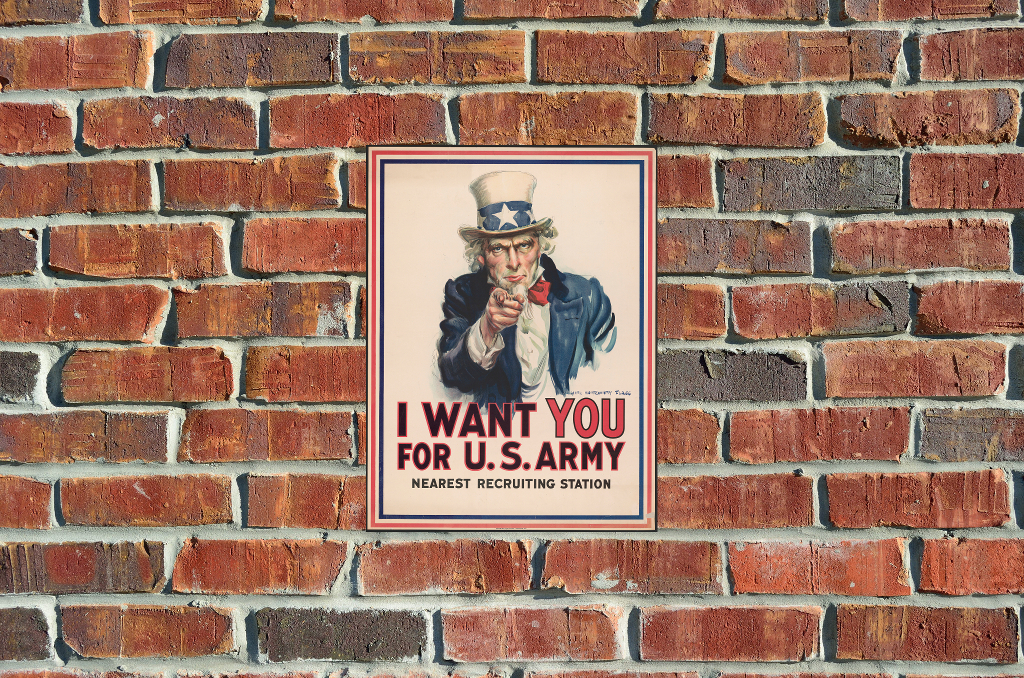
\includegraphics[width=7.5cm]{img/examples/wall.jpg}
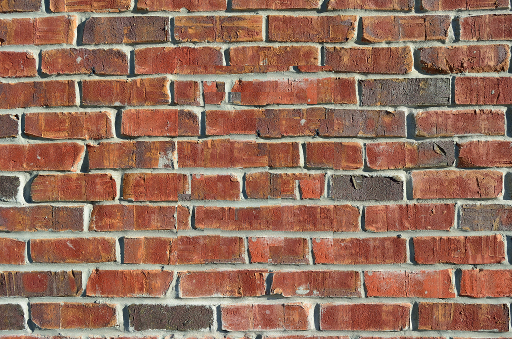
\includegraphics[width=7.5cm]{img/examples/wall_res.jpg}
\caption{Pas de flou, et des teintes conservées}
\end{figure}

\subsection{Rapidité relative et parallélisation}
L'algorithme remplit les zones à complèter avec des patchs. Cela signifie que
les pixels ne sont pas remplis un par un mais par groupes, donc l'algorithme
accélère grandement si on demande l'utilisation de patch plus grands.
De plus, l'étape la plus chronophage de l'algorithme est la recherche du 
patch de l'image d'origine qui est le plus proche de la zone à remplire.
En effet, il faut parcourir tous les pixels de l'image, et pour chaque
pixel tester la distance entre les patchs autour ce ce pixel. Cependant,
comme on cherche le patch minimisant la distance, on peut très facilement
paralléliser cette étape en répartissant les zones à tester sur les 
différents coeurs d'un processeur, ou utiliser la puissance d'une carte graphique
pour accélerer ce process.
Cet algorithme se parallélise donc très bien.

\subsection{Contrôle sur le grain}
Comme les patchs sont de taille fixée par l'utilisateur, ce dernier peut choisir
la taille adaptée à ses besoins. Un patch grand rendra l'algorithme plus rapide,
avec des zones cohérentes, et moins de frontières entre patchs, qui entrainent
souvent des démarcations plus ou moins visibles. Un patch plus petit prendra
plus de temps, mais donnera un grain plus fin, rendant certaines transitions
entre patchs moins visibles, mais plus nombreuses.

\begin{figure}[ht]
\centering
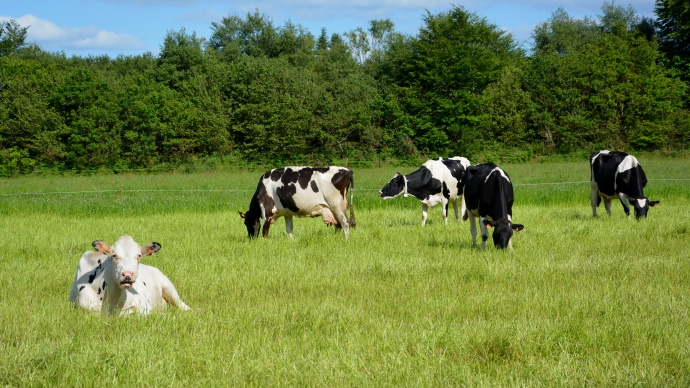
\includegraphics[width=7.5cm]{img/examples/vache.jpg}
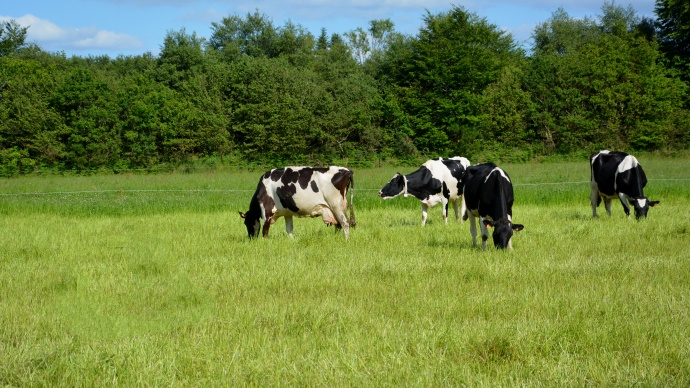
\includegraphics[width=7.5cm]{img/examples/vache_res.jpg}
\caption{Avec le bon grain, les délimitations ne sont pas visibles}
\end{figure}

\section{Inconvénients}
\subsection{Rapidité}
L'algorithme peut vite devenir très lent pour des patchs petits, remplissant lentement
la zone à remplire, et des images grandes, fournissant une grande zone où tester la 
distance entre les patchs.

\subsection{Résultat intermédiaire}
Pendant le déroulement de l'algorithme, on peut exporter l'image en partie remplie.
Cependant cette image aura toujours une grande zone noire, la zone à completer, alors
que d'autre algorithmes, travaillant sur tous les pixels à la fois peuvent avoir des
résultats intermédiaires plus utilisables.

\begin{figure}[ht]
\centering
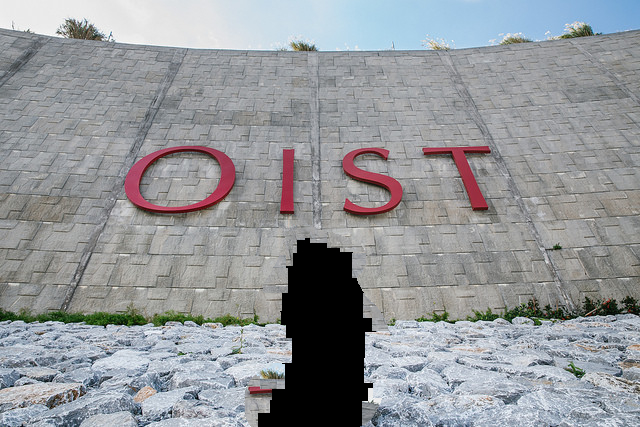
\includegraphics[width=7.5cm]{img/examples/inter.jpg}
\caption{Resultat intermédiaire}
\end{figure}

\subsection{Les lignes à continuer}
Dans la première section j'évoquais comment l'algo préférait continuer les lignes de fort
gradient, pour prolonger les formes. Cependant, cela pose problème dans des images
à très fort gradient, alors l'algorithme va s'engoufrer en suivant ces lignes mais cela
peut nuire à la cohérence globale de l'image, comme le montre l'image intermédiaire suivante.

\begin{figure}[ht]
\centering
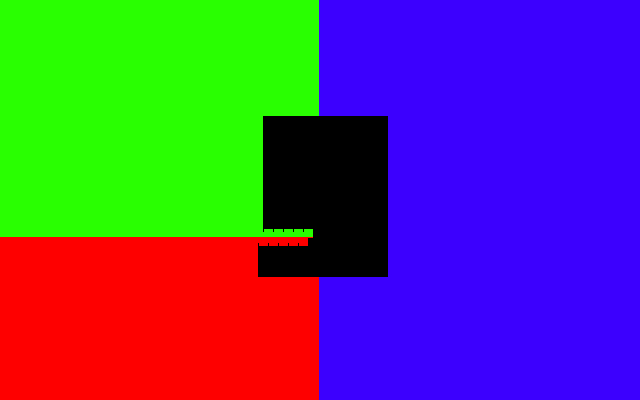
\includegraphics[width=7.5cm]{img/examples/line.jpg}
\caption{Suivre les lignes}
\end{figure}

\subsection{Grande dépendance au grain}
La taille du patch influe énormément sur le résultat de l'algorithme. Un patch trop grand
donnera des délimitations plus visibles et des détails incohérents, et un patch plus 
petit entrainera un temps d'exécution plus long, et parfois un manque de cohérence du 
résultat global. Localement l'image sera très cohérente, mais avec du recul on se rend 
compte du manque de cohérence du résultat.

\begin{figure}[ht]
\centering
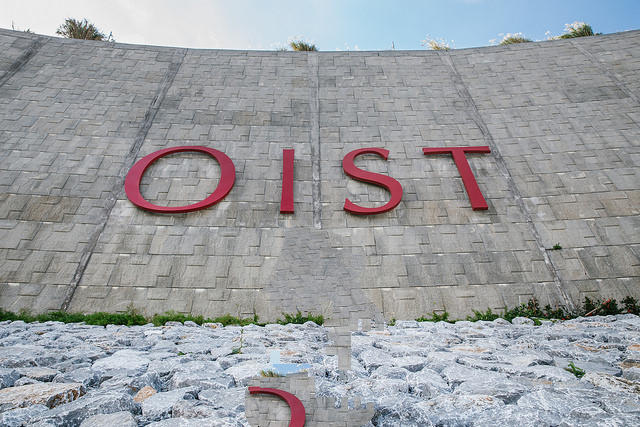
\includegraphics[width=7.5cm]{img/examples/big_patch.jpg}
\caption{Inpainting avec patchs trop grands}
\end{figure}



\begin{thebibliography}{9}
\bibitem{article}
  Object removal by exemplar-based inpainting,
  Criminisi, Antonio and Perez, Patrick and Toyama, Kentaro,
  Computer Vision and Pattern Recognition, 2003. Proceedings. 2003 IEEE Computer Society Conference on,
  2,
  II--II,
  2003,
  IEEE.

\end{thebibliography}

\end{document}
